%   % !TEX root = ../../VIII,3_Rahmen-TeX_9-0.tex
%  
%   Band VIII, 3 N.~?? 	
%   Signatur/Tex-Datei:	LH_35_09_16_017
%   RK-Nr. 	41167
%   edlabels: 			3
%   Diagramme: 		4
%   Dateien (PDF):
%   		LH_35_09_16_017_d1_017r;
%   		LH_35_09_16_017_d2_017v;
%   		LH_35_09_16_017_d3_017v;
%   		LH_35_09_16_017_d4_017v;
%
\selectlanguage{ngerman}
\frenchspacing
%
\begin{ledgroupsized}[r]{120mm}
\footnotesize
\pstart
\noindent\textbf{Überlieferung:}
\pend
\end{ledgroupsized}
%
\begin{ledgroupsized}[r]{114mm}
\footnotesize
\pstart \parindent -6mm
\makebox[6mm][l]{\textit{L}}%
Aufzeichnung:
LH~XXXV~9,~16 Bl.~17.
Ein als Schreibblatt wiederverwendeter Briefumschlag mit unregelmäßigen Rändern (ca.~17~x~12 cm.);
Wasserzeichenfragment am Blattrand;
geringfügiger Textverlust an den Rändern.
Zwei Seiten.
Auf Bl.~17~v\textsuperscript{o}, von Leibniz überschrieben, die fremdhändige Briefanschrift: \glqq\textit{A} \lbrack/\rbrack\ \textit{Monsieur} \lbrack/\rbrack\ \textit{Monsieur le Conseiller} \lbrack/\rbrack\ \textit{Leibnitz} \lbrack/\rbrack\ \textit{à} \lbrack/\rbrack\ \textit{Hannover}\protect\index{Ortsregister}{Hannover}\grqq.
\pend
\end{ledgroupsized}
%
%%
\selectlanguage{latin}
\frenchspacing
%
\vspace{8mm}
%
\pstart\noindent
\lbrack17~r\textsuperscript{o}\rbrack\
\pend
%
\vspace{2.0em} %Diagramm 1
\centerline{
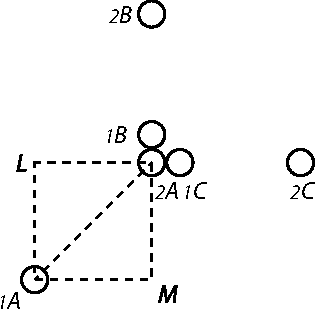
\includegraphics[width=0.33\textwidth]{gesamttex/edit_VIII,3/images/LH_35_09_16_017_d1_017r.pdf}}
\vspace{0.5em}
\centerline{%
\lbrack\textit{Fig.~1}\rbrack}
% \newpage%
\vspace{1.0em}
%
\pstart\noindent
\edtext{}{% 
\lemma{\hspace*{1,6mm}%
\lbrack\textit{Fig.~1}\rbrack%
}\killnumber%
\Cfootnote{%
Ein gestrichener Entwurf zum Diagramm wird nicht wiedergegeben.%
}}%
%%
\edtext{Si globus\protect\index{Sachverzeichnis}{globus}}{\lemma{Si}\Bfootnote{\textit{(1)}~corpus \textit{(2)}~globus~\textit{L}}}
%
\textit{A} ex loco \textit{{\scriptsize1}A} tendat in locum \textit{{\scriptsize2}A}, ibique
%
\edtext{incurrat in globos inter se et ipsi priori aequales\protect\index{Sachverzeichnis}{globi inter se aequales} nempe \textit{B} et \textit{C}, pondere pariter et volumine,}{%
\lemma{incurrat in}%
\Bfootnote{%
\textit{(1)}~corpo %
\textit{(2)}~globos inter se %
\textit{(a)}~aequales, et singulos ipsius \textit{A} dimidios, nempe \textit{B} et \textit{C}, %
ita ut ambo \textit{B} et \textit{C} simul primo \textit{A} sint aequales, 
\textit{(aa)}~tam pond
\textit{(bb)}~licet omnes tres inter se volumine aequales sint,
\textit{(b)}~et ipsi %
\textit{(aa)}~globo %
\textit{(bb)}~priori aequales
\textbar\ pondere \textit{streicht Hrsg.}~\textbar\ %
nempe \textit{B} et \textit{C}, pondere pariter %
\textit{(aaa)}~et volumine
\textit{(bbb)}~et volumine~\textit{L}}}
%
et ponamus \textit{{\scriptsize1}B}, \textit{{\scriptsize1}C}, \textit{{\scriptsize2}A} esse horum globorum centra,
%
et \textit{{\scriptsize1}B{\scriptsize2}A}, aequalem esse ipsi \textit{{\scriptsize1}C{\scriptsize2}A},
%
angulumque \edtext{\textit{{\scriptsize1}B}\lbrack\textit{{\scriptsize2}}\rbrack\textit{A{\scriptsize1}C}}{%
\lemma{}%
\Bfootnote{%
\textit{{\scriptsize1}B{\scriptsize1}A{\scriptsize1}C} % 
\textit{L ändert Hrsg.}}}
esse rectum\lbrack,\rbrack%
\protect\index{Sachverzeichnis}{angulus rectus}
%
ajo post ictum corpus \textit{A} quidem quieturum in loco \textit{{\scriptsize2}A}\lbrack,\rbrack\ 
%
corpora autem \textit{B} et \textit{C} recipere impetum,\protect\index{Sachverzeichnis}{impetus}
%
et \textit{B} quidem ex \textit{{\scriptsize1}B} tendere in \textit{{\scriptsize2}B},
%
linea \textit{{\scriptsize1}A{\scriptsize1}B{\scriptsize2}B} continuata, celeritate ea qua \textit{A} tendens 
%
ex \textit{{\scriptsize1}A} versus \textit{{\scriptsize2}A}, tendebat simul ex \textit{{\scriptsize1}A} versus~\textit{L},
%
\edtext{posito \textit{{\scriptsize 1}AL}}{%
\lemma{posito}%
\Bfootnote{%
\textit{(1)}~\textit{{\scriptsize 1}A} esse ipsi %
\textit{(2)}~\textit{{\scriptsize 1}AL}~\textit{L}}}
%
esse ipsi \edtext{\textit{{\scriptsize1}B{\scriptsize2}B} parallelam}{\lemma{\textit{{\scriptsize1}B{\scriptsize2}B}}\Bfootnote{\textit{(1)}~aequalem \textit{(2)}~parallelam~\textit{L}}}. 
%
\textit{C} vero similiter ex \textit{{\scriptsize1}C} tendere versus \textit{{\scriptsize2}C} celeritate ea
%
\edtext{qua \textit{A} tendens}{%
\lemma{qua \textit{A}}%
\Bfootnote{%
\textit{(1)}~ex %
\textit{(2)}~tendens~\textit{L}}}
%
ex \textit{{\scriptsize1}A} versus \textit{{\scriptsize2}A}, tendebat simul ex \textit{{\scriptsize1}A} versus \textit{M},
%
posito \textit{{\scriptsize1}AM} esse parallelam ipsi \textit{{\scriptsize1}C{\scriptsize2}C}. Ita
% 
\edtext{enim eadem}{\lemma{enim}\Bfootnote{\textit{(1)}~non \textit{(2)}~eadem~\textit{L}}} 
%
servatur quantitas \edtext{directionis\protect\index{Sachverzeichnis}{quantitas directionis} %
et virium;\protect\index{Sachverzeichnis}{quantitas virium}}{%
\lemma{directionis}%
\Bfootnote{%
\textit{(1)}~virium %
\textit{(2)}~et virium;~\textit{L}}}
%
\textso{directionis}\protect\index{Sachverzeichnis}{directio}\, %
quidem, quia centrum gravitatis commune\protect\index{Sachverzeichnis}{centrum gravitatis commune}
%
\edtext{omnium pergit in linea \textit{{\scriptsize1}A{\scriptsize2}A} eadem qua prius celeritate}{\lemma{omnium}\Bfootnote{\textit{(1)}~eadem vi \textit{(2)}~pergit~\textit{L}}}.
%
\textso{Virium}\protect\index{Sachverzeichnis}{vis}\,
%
autem, quia si ponamus ${\scriptstyle\textit{1}}B{\scriptstyle\textit{2}}B={\scriptstyle\textit{1}}AL$, 
%
et ${\scriptstyle\textit{1}}C{\scriptstyle\textit{2}}C={\scriptstyle\textit{1}}AM$,
%
\edtext{patet quadr. \textit{{\scriptsize1}B{\scriptsize2}B}}{\lemma{patet}\Bfootnote{\textit{(1)}~quadrata \textit{(a)}~rectarum \textit{(b)}~celeritatum \textit{(c)}~\textit{{\scriptsize1}B}\ \textit{(2)}~quadr.~\textit{L}}} 
%
(seu ${\scriptstyle1}AL)\ +\ \text{quadr.}\ {\scriptstyle1}C{\scriptstyle2}C$ (seu \textit{{\scriptsize1}AM}) esse aequal.\ quadrato \textit{{\scriptsize1}A{\scriptsize2}A}.
%
Ac proinde \edtext{ambo}{\lemma{}\Bfootnote{ambo \textit{erg.}~\textit{L}}} 
%
quadrata celeritatum\protect\index{Sachverzeichnis}{quadratum celeritatis}
%
\edtext{\lbrack post\rbrack}{%
\lemma{}%
\Bfootnote{%
ante %
\textit{L ändert Hrsg.}}}
%
concursum ducta in cuiuslibet corpus%
\protect\index{Sachverzeichnis}{quadratum celeritatis ductum in corpus}
%
(\protect\vphantom)nempe qu.\ \textit{{\scriptsize1}B{\scriptsize2}B} in \textit{B},\ +\ 
%
\edtext{\lbrack qu.\rbrack}{%
\lemma{}%
\Bfootnote{%
qu. %
\textit{erg.~Hrsg.}}}
%
\textit{{\scriptsize1}C{\scriptsize2}C} in \textit{C}\protect\vphantom()
%
aequari quadrato celeritatis ante concursum, in suum corpus%
\protect\index{Sachverzeichnis}{quadratum celeritatis ductum in corpus} %
(seu qu.\ \edtext{\textit{{\scriptsize1}A{\scriptsize2}A} in \textit{A}).}{\lemma{\textit{{\scriptsize1}A{\scriptsize2}A}}\Bfootnote{\textit{(1)}~in \textit{{\scriptsize1}A} \textit{(2)}~in \textit{(3)}~in \textit{A}\phantom(\hspace*{-1.2mm}).~\textit{L}}}
%
\edlabel{35_09_16_017_3a}% 
\edtext{Hinc patet compositiones motuum% 
\protect\index{Sachverzeichnis}{compositio motuum in angulo recto}
%
\edtext{in angulo recto\protect\index{Sachverzeichnis}{angulus rectus}}{\lemma{}\Bfootnote{in angulo recto \textit{erg.}~\textit{L}}}
%
praeclare conciliari cum principio aestimandarum 
%
\edtext{virium\protect\index{Sachverzeichnis}{principium aestimandarum virium} %
a quadratis celeritatum%
\protect\index{Sachverzeichnis}{quadratum celeritatis} seu altitudinibus}{%
\lemma{virium a}%
\Bfootnote{%
\textit{(1)}~quadrato celeritatum seu altitudine %
\textit{(2)}~quadratis celeritatum seu altitudinibus~\textit{L}}}
% %%% A-Fn mit viertem Apparat
spatiorum. Non vero cum principio aestimandi per quantitatem}{%
\lemma{}\Afootnote{\textit{Am unteren rechten Rand, quer zur Schreibrichtung}: %
NB Hic ostensum quod compositioni motuum\protect\index{Sachverzeichnis}{compositio motuum} %
non fidendum nisi quat.\ conciliatur compositioni virium\lbrack,\rbrack\protect\index{Sachverzeichnis}{compositio virium} %
quod fit in angulo recto,\protect\index{Sachverzeichnis}{angulus rectus} et quomodo per %
\textso{methodum alternorum}\textsuperscript{\lbrack a\rbrack}\protect\index{Sachverzeichnis}{methodus alternorum} %
seu elective concurrentium\protect\index{Sachverzeichnis}{methodus elective concurrentium} %
in angulo obliquo\protect\index{Sachverzeichnis}{angulus obliquus} problema %
solvas.%
\newline\newline%Marginalienapparat
{\footnotesize\textsuperscript{\lbrack a\rbrack} per \textso{methodum alternorum}:\enskip Zur Formulierung der \glqq regula alternativorum\grqq\ siehe \textsc{G.\,W.\,Leibniz}, \cite{01098}\glqq Demonstratio geometrica regulae apud Staticos receptae\grqq, in \cite{01023}\textit{AE}, November 1685, S.~501\textendash505, hier S.~503\textendash505. Das Stück erscheint in einem späteren Band der Reihe.}%
}}%
\edlabel{35_09_16_017_3b} 
%
\edlabel{35_09_16_017_1a}%
\edtext{}{% 
{\xxref%
{35_09_16_017_1a}{35_09_16_017_1b}}%
\lemma{motus.}%
\Bfootnote{%
\lbrack17~v\textsuperscript{o}\rbrack\ 
\textit{(1)}~Si corpora concurrentia sint inaequalia, vel si celeritat\textlangle es\textrangle\ %
\textit{(2)}~Si corpora~\textit{L}}}%
motus.\protect\index{Sachverzeichnis}{principium aestimandi per quantitatem motus}
\pend
%
\pstart
\lbrack17~v\textsuperscript{o}\rbrack\ Si corpora%
\edlabel{35_09_16_017_1b} %
%
concurrentia sint inaequalia; eodem modo facile habebitur calculus efficiendo ut tam linea centri gravitatis%
\protect\index{Sachverzeichnis}{linea centri gravitatis}
%
 quam vires serventur; nec refert, etiamsi
\textit{{\scriptsize1}AL}
et \textit{{\scriptsize1}AM}
sint inaequales inter se.
\pend
%
\vspace{2.0em} %Diagramm 2
\centerline{%
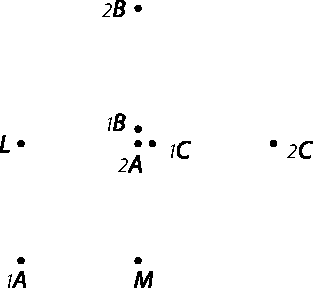
\includegraphics[width=0.33\textwidth]{%
gesamttex/edit_VIII,3/images/LH_35_09_16_017_d2_017v.pdf%
}} 
\vspace{0.5em}
\centerline{%
\lbrack\textit{Fig.~2}\rbrack%
}
% \newpage%
\vspace{1.5em}
%
\centerline{%
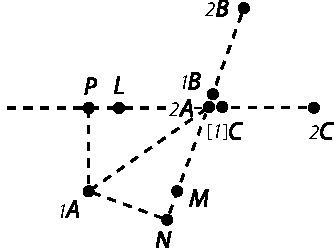
\includegraphics[width=0.33\textwidth]{%
gesamttex/edit_VIII,3/images/LH_35_09_16_017_d3_017v.pdf%
}} 
\vspace{0.5em}
\centerline{%
\lbrack\textit{Fig.~3}\rbrack%
}
%
\pstartfirst
Verum illud 
%
\edtext{plurimum refert,}{\lemma{}\Bfootnote{plurimum \textbar\ refert \textit{streicht Hrsg.}~\textbar\ refert,~\textit{L}}}
%
utrum angulus sit rectus.\protect\index{Sachverzeichnis}{angulus rectus} Nam si angulus \textit{BAC} sit obliquus,%
\protect\index{Sachverzeichnis}{angulus obliquus}
%
tunc \edtext{quidem directio}{\lemma{}\Bfootnote{quidem \ \textbar\ servabitur \textit{streicht Hrsg.}~\textbar \ directio~\textit{L}}}
%
centri gravitatis%
\protect\index{Sachverzeichnis}{directio centri gravitatis}
%
 servabitur. Sed non potest fieri ut eo tempore perveniant \textit{B} in \textit{{\scriptsize2}B}, et \textit{C} in \textit{{\scriptsize2}C},
%
quo \textit{A} venerat ex \textit{{\scriptsize1}A} in \textit{{\scriptsize2}A} posito parallelogrammum%
\protect\index{Sachverzeichnis}{parallelogrammum} \textit{L{\scriptsize1}AM}
%
parallelogrammo \textit{{\scriptsize 2}A{\scriptsize 2}B{\scriptsize 2}C}
%
(\phantom)\hspace*{-1.2mm}si \textit{{\scriptsize 2}A}, \textit{{\scriptsize 1}C}, \edtext{\lbrack\textit{{\scriptsize 1}B}\rbrack}{%
\lemma{}%
\Bfootnote{%
\textit{{\scriptsize 2}B} %
\textit{L ändert Hrsg.}}}
coincidere ponantur\phantom(\hspace*{-1.2mm})
%
esse aequale et simile, nam tunc quadrata \textit{{\scriptsize1}B{\scriptsize2}B} et  \textit{{\scriptsize1}C{\scriptsize2}C}
%
forent utique majora quadrato \textit{{\scriptsize1}A{\scriptsize1}C}, ergo major prodiret vis\protect\index{Sachverzeichnis}{vis}
%
quam ante\lbrack,\rbrack\
% 
\edtext{quare non tuto}{\lemma{quare}\Bfootnote{\textit{(1)}~quadrato virium \textit{(2)}~non tuto~\textit{L}}}
%
fiditur compositioni
%
\edtext{motuum.\protect\index{Sachverzeichnis}{compositio motuum} Sed}{\lemma{motuum}\Bfootnote{\textit{(1)}~, nisi \textit{(2)}~. Sed~\textit{L}}}
%
res ad aestimationem virium%
\protect\index{Sachverzeichnis}{aestimatio virium}
%
 est revocanda. Itaque
%
\edtext{in \textit{MB} productam}{\lemma{in}\Bfootnote{\textit{(1)}~\textit{{\scriptsize1}A} productam \textit{(2)}~\textit{MB} productam~\textit{L}}}
%
demittatur ex \textit{{\scriptsize1}A} perpendicularis \textit{{\scriptsize1}AN}. Constat \textit{{\scriptsize1}A}
%
celeritate \textit{{\scriptsize1}A{\scriptsize2}A} ipsi \textit{{\scriptsize1}B} imprimere celeritatem\protect\index{Sachverzeichnis}{celeritas}
%
et directionem\protect\index{Sachverzeichnis}{directio}
%
\textit{{\scriptsize1}B{\scriptsize2}B} quae sit aequalis ipsi \textit{N{\scriptsize2}A}, et similiter
%
ex \textit{{\scriptsize1}A} in \textit{LC} perpendicularis ducatur \textit{{\scriptsize1}AP}. Patet similiter \textit{{\scriptsize1}A} celeritate
%
\textit{{\scriptsize1}A{\scriptsize2}A} ipsi \textit{{\scriptsize1}C} imprimere celeritatem \textit{{\scriptsize1}C{\scriptsize2}C} ipsi 
%
\edtext{\lbrack\textit{{\scriptsize 2}AP}\rbrack}{%
\lemma{}%
\Bfootnote{%
\textit{{\scriptsize 1}A{\scriptsize 1}P} %
\textit{L ändert Hrsg.}}}
%
aequalem\lbrack,\rbrack\ \edlabel{35_09_16_017_2a}%
si scilicet singula % 
%
corpora \textit{B} vel \textit{C} sola essent cum corpore \textit{A}, sed cum nunc ambo \edtext{a\lbrack d\rbrack sint}{%
\lemma{}%
\Bfootnote{%
absint %
\textit{L ändert Hrsg.}}}
%
foret effectus major causa.\protect\index{Sachverzeichnis}{effectus major causa}%
\edlabel{35_09_16_017_2b} 
%
Ergo in \edtext{quantum quadr.\ $P{\scriptstyle\textit{2}}A\ +\ \text{quadr.}\ N{\scriptstyle\textit{2}}A$}{\lemma{quantum}\Bfootnote{\textit{(1)}~$\text{quadr.}\ PC\ +\ \text{quadr.}$ \textit{(2)}~$P{\scriptstyle\textit{2}}A\ +\ \text{quadr.}\ N{\scriptstyle\textit{2}}A$~\textit{L}}}
% 
majus est quadrato \textit{{\scriptsize1}A{\scriptsize2}A} in tantum qu.\ \textit{N{\scriptsize2}A} erit majus
%
quadrato \textit{{\scriptsize1}B{\scriptsize2}B}, et quadratum \textit{P{\scriptsize2}A} majus quadrato \textit{{\scriptsize1}C{\scriptsize2}C}. 
%
Prorsus ut 
%
\edtext{in meo Schediasmate circa planum
\edtext{inclinatum\protect\index{Sachverzeichnis}{planum inclinatum} \cite{01023}\textit{Actis} Lips.}{\lemma{inclinatum}\Bfootnote{%
\textit{(1)}~\textit{Actis} inserto \textit{(2)}~\textit{Act} \textit{(3)}~\textit{Actis} Lips.~\textit{L}}}
1686 inserto.}{%
\lemma{in meo \lbrack...\rbrack\ 1686 inserto}\Cfootnote{\cite{01098}a.a.O., bes.\ S.~503\textendash505. Der Aufsatz war eigentlich in den \cite{01023}\textit{Acta Eruditorum} vom November 1685 erschienen; siehe die Vorbemerkung zu N.~\ref{comp_non_fidendum}.}}
\pend
%
\pstart
\textso{Methodus} hic \textso{concursuum}\protect\index{Sachverzeichnis}{methodus concursuum}\, 
%
ut \edtext{in jure accrescendi,\protect\index{Sachverzeichnis}{jus accrescendi}}{\lemma{}\Afootnote{%
\textit{Über dem Text, bezogen auf} in jure accrescendi:\enskip Simile specimen in \cite{01023}\textit{Actis} Lips.\ dedi, ubi de gravi %
plana duo inclinata inter se recta\protect\index{Sachverzeichnis}{plana duo inclinata inter se recta} %
premente.\textsuperscript{\lbrack a\rbrack}
\newline%
\textit{Darüber, bezogen auf} \textso{Methodus} hic \textso{concursuum}\, \textit{und auf S.~\refpassage{35_09_16_017_2a}{35_09_16_017_2b}:} NB.~NB.\ \textso{Non succedit hoc loco.} %
\newline\newline %Marginalienapparat:
{\footnotesize \textsuperscript{\lbrack a\rbrack} specimen \lbrack...\rbrack\ premente: \cite{01098}a.a.O., bes.\ S.~502\textendash504.}}}
%
quid \edtext{scilicet}{%
\lemma{}%
\Bfootnote{%
scilicet %
\textit{erg.~L}}}
%
dicendum de duobus quando constat de singulis si sola essent,
%
sed ambo simul sic consistere non possunt,
%
quantitate distribuenda non s\textlangle olum cele\textrangle ritate.
%
\edtext{}{% Trick für Anm. zu Diagramm 4
\lemma{\hspace*{1,6mm}%
\lbrack\textit{Fig.~4}\rbrack%
}\killnumber%
\Cfootnote{%
Ein gestrichener Entwurf zum Diagramm wird nicht wiedergegeben.%
}}
\pend
%
\vspace{1.5em} % Diagramm 4
\centerline{%
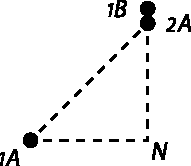
\includegraphics[width=0.20\textwidth]{%
gesamttex/edit_VIII,3/images/LH_35_09_16_017_d4_017v.pdf%
}} 
\vspace{0.5em}
\centerline{%
\lbrack\textit{Fig.~4}\rbrack%
}
\count\Afootins=1200%
\count\Bfootins=1200%
\count\Cfootins=1200